\section{学生讲义：晶体结构基础（超级充实版）}\label{ux5b66ux751fux8bb2ux4e49ux6676ux4f53ux7ed3ux6784ux57faux7840ux8d85ux7ea7ux5145ux5b9eux7248}

\begin{center}\rule{0.5\linewidth}{0.5pt}\end{center}

\subsection{学习目标}\label{ux5b66ux4e60ux76eeux6807}

\begin{itemize}
\tightlist
\item
  能说出晶体的微观定义（点阵+结构基元），理解晶胞是最小重复单元
\item
  能根据轴长/轴角判断7大晶系，知道14种布拉维格子的存在
\item
  能完整推导ccp/hcp/bcc的空间利用率，计算空隙类型与数目
\item
  能用半径比规则预测 NaCl 型、CsCl 型、ZnS 型结构，并理解临界值的几何来源
\item
  能理解 Pauling 电价规则和离子极化导致的键型过渡（如 AgI 从 NaCl 型→ZnS 型）
\item
  能用''负离子骨架 + 正离子填隙 + 配位多面体''语言解释常见离子晶体结构
\item
  能区分离子/原子/分子/金属晶体的键型、特征实例和典型物性
\end{itemize}

\begin{center}\rule{0.5\linewidth}{0.5pt}\end{center}

\subsection{一、晶体学基础}\label{ux4e00ux6676ux4f53ux5b66ux57faux7840}

\textbf{关联知识点}：晶体结构 · 晶体基本概念 · 晶体与非晶体 · 点阵与晶胞

\subsubsection{1.1 什么是晶体？------从宏观现象到微观本质}\label{ux4ec0ux4e48ux662fux6676ux4f53ux4eceux5b8fux89c2ux73b0ux8c61ux5230ux5faeux89c2ux672cux8d28}

食盐为什么是方方正正的立方体？雪花为什么是六角形的？钻石为什么是所有天然矿物中最硬的？这些问题看似分散，但答案都指向同一个事实：\textbf{这些物质的原子/离子/分子在三维空间中呈周期性重复排列}。这样的固体，就是晶体的本质。

\begin{quote}
🧠 \textbf{认知对比}：「晶体 vs 非晶体」------晶体像图书馆里的书（每本书在固定的书架上、固定的位置，取走一本，另一本也是同样的方向放在那里），非晶体像垃圾场里的杂物（随意堆叠，没有长程周期）。普通玻璃是典型的非晶体------它没有固定的熔点，只是逐渐软化。
\end{quote}

\textbf{晶体} = \textbf{点阵} + \textbf{结构基元}

\begin{itemize}
\tightlist
\item
  \textbf{点阵}：在空间无限排列的、周围环境相同的几何点
\item
  \textbf{结构基元}：重复排列的基本结构单元（原子/离子/分子）。基元可以包含多个原子------只要它们的排列方式完全相同
\item
  \textbf{晶胞}：晶体结构的最小重复单元，整个晶体可由晶胞在三维空间平移复制得到
\end{itemize}

\begin{figure}[H]\centering
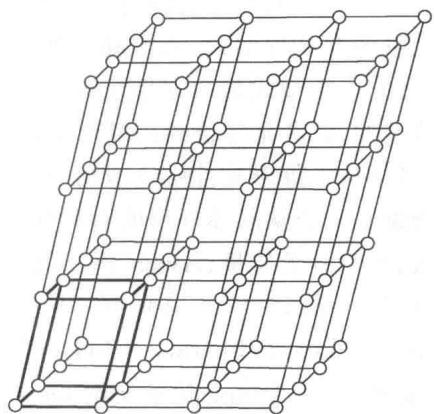
\includegraphics[width=0.9\textwidth,keepaspectratio]{media/spatial-lattice.jpg}
\caption{图1 空间点阵示意图 — 原子在三维空间作周期性排列。左：抽象点阵点；右：实际原子排布}
\end{figure}

\begin{quote}
⚠️ \textbf{易错点}：结构基元 ≠ 晶胞 ≠ 一个原子。结构基元是''内容''（含什么+怎么排），点阵是''框架''（几何位置关系）。干冰的结构基元含4个CO\textsubscript{2}分子------因为4个分子的取向不同，取其中1个平移无法还原整个晶体。
\end{quote}

\textbf{晶体的五个基本性质}：自范性、各向异性、对称性、固定熔点、均一性

\subsubsection{1.2 七大晶系------晶体分类的''骨架''}\label{ux4e03ux5927ux6676ux7cfbux6676ux4f53ux5206ux7c7bux7684ux9aa8ux67b6}

根据晶胞的\textbf{轴长 a、b、c} 和\textbf{轴角 α、β、γ}，晶体可分为7大晶系。但注意：\textbf{晶系由特征对称元素决定，不是由晶胞参数数值决定的}。

\begin{quote}
🧠 \textbf{认知冲突}：「为什么晶体没有5次对称轴？」------数学证明表明，周期排列只能允许1/2/3/4/6次旋转轴。五边形不能无空隙地铺满平面→晶体中不可能出现5次对称。这就是''轴次定理''。
\end{quote}

{\def\LTcaptype{none} % do not increment counter
\begin{longtable}[]{@{}
  >{\raggedright\arraybackslash}p{(\linewidth - 8\tabcolsep) * \real{0.2000}}
  >{\raggedright\arraybackslash}p{(\linewidth - 8\tabcolsep) * \real{0.2000}}
  >{\raggedright\arraybackslash}p{(\linewidth - 8\tabcolsep) * \real{0.2000}}
  >{\raggedright\arraybackslash}p{(\linewidth - 8\tabcolsep) * \real{0.2000}}
  >{\raggedright\arraybackslash}p{(\linewidth - 8\tabcolsep) * \real{0.2000}}@{}}
\toprule\noalign{}
\begin{minipage}[b]{\linewidth}\raggedright
晶系
\end{minipage} & \begin{minipage}[b]{\linewidth}\raggedright
轴长关系
\end{minipage} & \begin{minipage}[b]{\linewidth}\raggedright
轴角关系
\end{minipage} & \begin{minipage}[b]{\linewidth}\raggedright
特征对称元素
\end{minipage} & \begin{minipage}[b]{\linewidth}\raggedright
实例
\end{minipage} \\
\midrule\noalign{}
\endhead
\bottomrule\noalign{}
\endlastfoot
\textbf{立方} & \(a = b = c\) & \(\alpha = \beta = \gamma = 90^\circ\) & 4个三重轴（体对角线方向） & NaCl、Cu、金刚石 \\
\textbf{四方} & \(a = b \neq c\) & \(\alpha = \beta = \gamma = 90^\circ\) & 1个四重轴 & TiO\textsubscript{2}（金红石） \\
\textbf{正交} & \(a \neq b \neq c\) & \(\alpha = \beta = \gamma = 90^\circ\) & 3个互相垂直的二重轴 & I\textsubscript{2}、HgCl\textsubscript{2} \\
\textbf{六方} & \(a = b \neq c\) & \(\alpha = \beta = 90^\circ, \gamma = 120^\circ\) & 1个六重轴 & 石墨、Mg \\
\textbf{三方（菱方）} & \(a = b = c\) & \(\alpha = \beta = \gamma \neq 90^\circ\) & 1个三重轴 & 方解石 CaCO\textsubscript{3} \\
\textbf{单斜} & \(a \neq b \neq c\) & \(\alpha = \gamma = 90^\circ, \beta \neq 90^\circ\) & 1个二重轴 & KClO\textsubscript{3} \\
\textbf{三斜} & \(a \neq b \neq c\) & \(\alpha \neq \beta \neq \gamma \neq 90^\circ\) & 无（只有对称中心） & CuSO\textsubscript{4}·5H\textsubscript{2}O \\
\end{longtable}
}

\begin{figure}[H]\centering
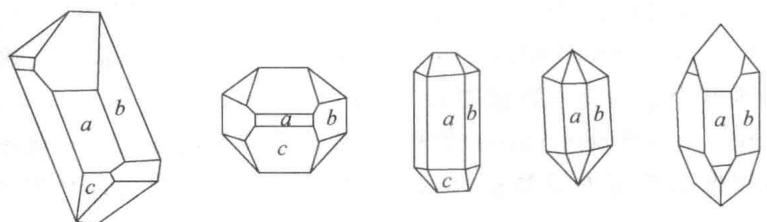
\includegraphics[width=0.9\textwidth,keepaspectratio]{media/13-1-quartz-crystal-faces-angle-constancy.jpg}
\caption{图2 石英晶体——天然晶体的规则外形反映了内部周期排列。晶体学的基本假设：不同产地、不同大小的同一矿物，对应晶面之间的夹角恒等}
\end{figure}

\begin{quote}
📝 \textbf{练一练}：已知某晶体的晶胞参数为 \(a = b = 0.52\ \mathrm{nm}, c = 0.68\ \mathrm{nm}, \alpha = \beta = 90^\circ, \gamma = 120^\circ\)，它属于什么晶系？
（答案见§九参考答案）
\end{quote}

\subsubsection{1.3 14种布拉维格子}\label{ux79cdux5e03ux62c9ux7ef4ux683cux5b50}

在7大晶系的基础上，考虑\textbf{带心方式}（P = 简单、I = 体心、F = 面心、C = 底心），共14种布拉维格子。这是晶体学中所有可能的点阵类型------\textbf{任何晶体结构都可以归为某一种布拉维格子}。

\begin{figure}[H]\centering
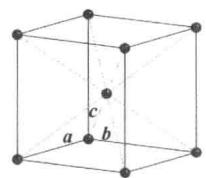
\includegraphics[width=0.9\textwidth,keepaspectratio]{media/13-3a-bravais-lattice-primitive-body-face-centered.jpg}
\caption{图3 布拉维格子示意图 — 从左至右：简单(P) 体心(I) 面心(F) 底心(C)}
\end{figure}

\begin{quote}
🗣️ \textbf{课堂原话}：``14种布拉维格子就像26个字母------用它们可以拼出所有晶体结构。第一轮不用全背，但要理解它的逻辑：晶系（7种）× 带心方式（最多4种）= 所有可能的几何组合。''
\end{quote}

相关 KP：七大晶系 · 点阵与晶胞 · 晶胞 · 晶系与对称性 · 布拉维格子

\begin{center}\rule{0.5\linewidth}{0.5pt}\end{center}

\subsection{二、金属密堆积}\label{ux4e8cux91d1ux5c5eux5bc6ux5806ux79ef}

\textbf{关联知识点}：密堆积 · 金属晶体 · 配位数

\subsubsection{2.1 为什么金属原子要''挤''在一起？}\label{ux4e3aux4ec0ux4e48ux91d1ux5c5eux539fux5b50ux8981ux6324ux5728ux4e00ux8d77}

金属原子的核外电子分布决定了它们倾向于以\textbf{尽可能密集}的方式排列------因为密集排列时原子间的距离最小，金属键（自由电子气与正离子实之间的静电吸引）最强，体系能量最低。所以绝大多数金属晶体的结构，就是\textbf{等径圆球的最密堆积}。

\subsubsection{2.2 四种基本堆积方式}\label{ux56dbux79cdux57faux672cux5806ux79efux65b9ux5f0f}

\begin{figure}[H]\centering
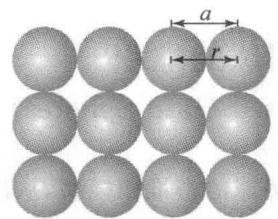
\includegraphics[width=0.9\textwidth,keepaspectratio]{media/13-7a-simple-cubic-packing-layer-top-view.jpg}
\caption{图4 简单立方堆积（sc）俯视图——每层球对齐排布，非最紧密排列}
\end{figure}

{\def\LTcaptype{none} % do not increment counter
\begin{longtable}[]{@{}cccccl@{}}
\toprule\noalign{}
堆积类型 & 符号 & 配位数 & 晶胞原子数 & 空间利用率 & 实例 \\
\midrule\noalign{}
\endhead
\bottomrule\noalign{}
\endlastfoot
简单立方 & sc & 6 & 1 & 52.36\% & Po（钋） \\
体心立方 & bcc / A2 & 8 & 2 & 68.02\% & Fe、Na、K、Cr \\
面心立方 & fcc / ccp / A1 & 12 & 4 & 74.05\% & Cu、Ag、Au、Al \\
六方密堆积 & hcp / A3 & 12 & 2 & 74.05\% & Mg、Zn、Ti、Co \\
\end{longtable}
}

\begin{figure}[H]\centering
\includegraphics[width=0.9\textwidth,keepaspectratio]{media/金属晶体A1A2A3对比.并列对比.png}
\caption{图12 金属晶体A1/A2/A3并列对比 — 三种基本堆积方式（fcc/bcc/hcp）的参数与实例一览}
\end{figure}

\begin{figure}[H]\centering
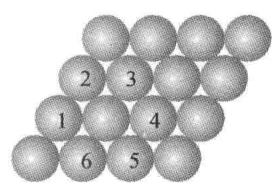
\includegraphics[width=0.9\textwidth,keepaspectratio]{media/close-packed-layer.jpg}
\caption{图5 密置层 — 等径圆球最紧密排列，每个球周围有6个球紧密接触。三个球之间的凹陷处形成两种三角形空隙（顶点向上/向下）}
\end{figure}

\begin{quote}
🧠 \textbf{认知冲突}：「为什么ccp和hcp的堆积系数都是74.05\%，但晶系不同？」------两者的差异不在堆积密度，而在\textbf{堆积层序}：ccp是ABCABC\ldots（三层一循环，产生立方对称性），hcp是ABAB\ldots（两层一循环，六方对称性）。\textbf{同样的密度，不同的排列方式}。
\end{quote}

\begin{quote}
🗣️ \textbf{课堂原话}：``CCP=ABC, HCP=AB, 密度一样高，堆法各不同。第三层去了新位置是CCP（立方），回到原位是HCP（六方）。''
\end{quote}

\begin{figure}[H]\centering
\includegraphics[width=0.9\textwidth,keepaspectratio]{media/密堆积-二维到三维.递进图.png}
\caption{图13 二维密置层→三维密堆积的演化过程 — 从单层到AB双层再到ABC/ABA分支}
\end{figure}

\subsubsection{2.3 空间利用率全推导}\label{ux7a7aux95f4ux5229ux7528ux7387ux5168ux63a8ux5bfc}

\textbf{关键思路}：空间利用率 = \(\frac{\text{晶胞中所有原子体积之和}}{\text{晶胞体积}} = \frac{Z \times \frac{4}{3}\pi r^3}{a^3}\)
核心步骤：① 找出原子接触方向 ② 用原子半径 r 表示晶胞参数 a ③ 代入公式计算

\paragraph{2.3.1 面心立方（fcc/ccp）}\label{ux9762ux5fc3ux7acbux65b9fccccp}

\textbf{原子接触方向}：面对角线方向（因为面心原子与顶点原子相切）

\(\sqrt{2}a = 4r\) → \(a = 2\sqrt{2}r\)

\textbf{晶胞原子数}：顶点 \(8 \times 1/8 = 1\) + 面心 \(6 \times 1/2 = 3\) = \textbf{4个}

\[
\text{空间利用率} = \frac{4 \times \frac{4}{3}\pi r^3}{(2\sqrt{2}r)^3} = \frac{16\pi r^3 / 3}{16\sqrt{2}r^3} = \frac{\pi}{3\sqrt{2}} \approx 74.05\%
\]

\paragraph{2.3.2 体心立方（bcc）}\label{ux4f53ux5fc3ux7acbux65b9bcc}

\textbf{原子接触方向}：体对角线方向（体心原子与顶点原子相切）

\(\sqrt{3}a = 4r\) → \(a = \frac{4r}{\sqrt{3}}\)

\textbf{晶胞原子数}：顶点 \(8 \times 1/8 = 1\) + 体心 \(1\) = \textbf{2个}

\[
\text{空间利用率} = \frac{2 \times \frac{4}{3}\pi r^3}{(4r/\sqrt{3})^3} = \frac{8\pi r^3 / 3}{64r^3 / 3\sqrt{3}} = \frac{\sqrt{3}\pi}{8} \approx 68.02\%
\]

\paragraph{2.3.3 六方密堆积（hcp）}\label{ux516dux65b9ux5bc6ux5806ux79efhcp}

\textbf{原子接触方向}：a轴方向（底面正六边形边长 = 2r），c轴方向的层间距决定理想轴比

底面正六边形面积：\(S = \frac{3\sqrt{3}}{2}a^2 = \frac{3\sqrt{3}}{2}(2r)^2 = 6\sqrt{3}r^2\)

理想轴比（两层之间的垂直距离 = 两个正四面体的高）：\(c = 2 \times \sqrt{\frac{2}{3}}a = 4\sqrt{\frac{2}{3}}r\)

\[
V = S \times c = 6\sqrt{3}r^2 \times 4\sqrt{\frac{2}{3}}r = 24\sqrt{2}r^3
\]

\textbf{晶胞原子数}：12个顶点各1/6（简单六方中）→ 晶胞含2个原子

\[
\text{空间利用率} = \frac{2 \times \frac{4}{3}\pi r^3}{24\sqrt{2}r^3} = \frac{\pi}{3\sqrt{2}} \approx 74.05\%
\]

\begin{quote}
📝 \textbf{练一练}：推导hcp的理想轴比 \(c/a\)。提示：密置双层中，上层球正好落在下层三个球围成的凹陷处，构成正四面体。两层球的球心垂直距离 = 正四面体的高 = \(\sqrt{6}/3 \times\) 边长。
（答案见§九参考答案）
\end{quote}

\begin{figure}[H]\centering
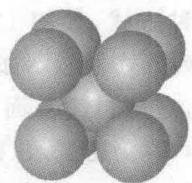
\includegraphics[width=0.9\textwidth,keepaspectratio]{media/13-7-10-four-unit-cell-types-sc-bcc-fcc.jpg}
\caption{图6 四种晶胞对比 — 简单立方（左上）、体心立方（右上）、面心立方（右下）及原子接触方向}
\end{figure}

\begin{figure}[H]\centering
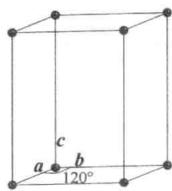
\includegraphics[width=0.9\textwidth,keepaspectratio]{media/13-7-10-unit-cell-types-sc-bcc-fcc-comparison.jpg}
\caption{图7 晶胞参数与原子半径关系对比图 — 从左至右：sc（棱边=2r）、bcc（体对角线=4r）、fcc（面对角线=4r）}
\end{figure}

\begin{figure}[H]\centering
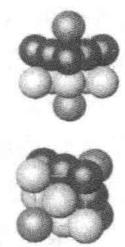
\includegraphics[width=0.9\textwidth,keepaspectratio]{media/ccp-unit-cell.jpg}
\caption{图8 面心立方（左）与体心立方（右）晶胞}
\end{figure}

\subsubsection{2.4 空隙分析}\label{ux7a7aux9699ux5206ux6790}

金属堆积中，原子之间不可避免会留下空隙（即使是最密堆积）。这些空隙是理解离子晶体结构的钥匙------\textbf{正离子就是填充在负离子堆积形成的空隙中}。

{\def\LTcaptype{none} % do not increment counter
\begin{longtable}[]{@{}
  >{\centering\arraybackslash}p{(\linewidth - 6\tabcolsep) * \real{0.2632}}
  >{\centering\arraybackslash}p{(\linewidth - 6\tabcolsep) * \real{0.2632}}
  >{\centering\arraybackslash}p{(\linewidth - 6\tabcolsep) * \real{0.2632}}
  >{\raggedright\arraybackslash}p{(\linewidth - 6\tabcolsep) * \real{0.2105}}@{}}
\toprule\noalign{}
\begin{minipage}[b]{\linewidth}\centering
堆积类型
\end{minipage} & \begin{minipage}[b]{\linewidth}\centering
四面体空隙数
\end{minipage} & \begin{minipage}[b]{\linewidth}\centering
八面体空隙数
\end{minipage} & \begin{minipage}[b]{\linewidth}\raggedright
说明
\end{minipage} \\
\midrule\noalign{}
\endhead
\bottomrule\noalign{}
\endlastfoot
\textbf{fcc/ccp} & 8（每个晶胞） & 4（每个晶胞） & 每个球对应 1 个八面体空隙 + 2 个四面体空隙 \\
\textbf{hcp} & 每个球对应 2 个 & 每个球对应 1 个 & 与 fcc 空隙数相同，但排列方式不同 \\
\textbf{bcc} & 无正四面体空隙 & 无正八面体空隙 & 空隙形状为非正多面体（变形的四面体/八面体） \\
\end{longtable}
}

\textbf{空隙数快速验证}：fcc 中，每个球周围有 8 个四面体空隙（4个在上方+4个在下方），但每个四面体空隙由 4 个球共享：\(8 \times 4 / 4 = 8\) 个四面体空隙。每个球周围有 6 个八面体空隙，每个由 6 个球共享：\(6 \times 4 / 6 = 4\) 个八面体空隙。✔️

\begin{figure}[H]\centering
\includegraphics[width=0.9\textwidth,keepaspectratio]{media/空隙-四面体八面体.标注图.png}
\caption{图14 四面体空隙与八面体空隙的位置标注 — 空隙类型对比、计数公式与fcc应用实例}
\end{figure}

\begin{figure}[H]\centering
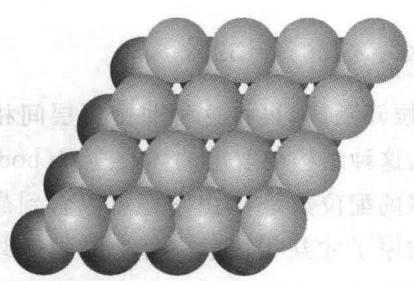
\includegraphics[width=0.9\textwidth,keepaspectratio]{media/13-8a-close-packed-bilayer-tetrahedral-octahedral-voids.jpg}
\caption{图9 密置双层中的空隙 —— 从双层俯视可见四面体空隙（T）和八面体空隙（O）的位置分布}
\end{figure}

\begin{figure}[H]\centering
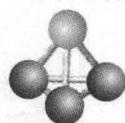
\includegraphics[width=0.9\textwidth,keepaspectratio]{media/13-8b-tetrahedral-void-structure.jpg}
\caption{图10 正四面体空隙（左）与正八面体空隙（右）—— 四面体空隙由4个等径球围成，八面体空隙由6个等径球围成}
\end{figure}

\begin{figure}[H]\centering
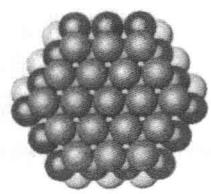
\includegraphics[width=0.9\textwidth,keepaspectratio]{media/ccp-stacking.jpg}
\caption{图11 面心立方密堆积 ABCABC…（左）与六方密堆积 ABAB…（右）层序对比}
\end{figure}

相关 KP：密堆积 · 金属晶体 · 配位数 · 简单立方堆积 · 立方密堆积 · 六方密堆积 · 体心立方堆积

\begin{center}\rule{0.5\linewidth}{0.5pt}\end{center}

\subsection{三、离子晶体结构类型}\label{ux4e09ux79bbux5b50ux6676ux4f53ux7ed3ux6784ux7c7bux578b}

\textbf{关联知识点}：离子晶体 · 离子半径

\subsubsection{3.1 为什么从金属堆积讲到离子晶体？}\label{ux4e3aux4ec0ux4e48ux4eceux91d1ux5c5eux5806ux79efux8bb2ux5230ux79bbux5b50ux6676ux4f53}

金属晶体是\textbf{等径球堆积}，但离子晶体不同------\textbf{负离子比正离子大得多}（通常2-3倍）。因此离子晶体的结构可以看作：

\textbf{负离子按一定方式堆积，正离子选择性填充在负离子围成的空隙中}

这就是''堆积-填隙''模型，是理解离子晶体最直观的语言。

\begin{figure}[H]\centering
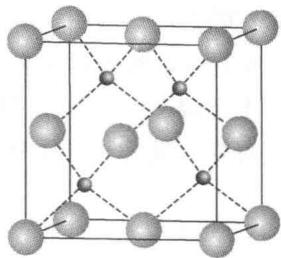
\includegraphics[width=0.9\textwidth,keepaspectratio]{media/13-11-three-ab-ionic-crystal-structures-nacl-cscl-zns.jpg}
\caption{图12 三种AB型离子晶体结构对比 —— 从左至右：NaCl型（6:6）、CsCl型（8:8）、ZnS型（4:4）}
\end{figure}

{\def\LTcaptype{none} % do not increment counter
\begin{longtable}[]{@{}llc@{}}
\toprule\noalign{}
负离子堆积方式 & 围成的空隙类型 & 配位数 \\
\midrule\noalign{}
\endhead
\bottomrule\noalign{}
\endlastfoot
简单立方 & 立方体空隙 & 8 \\
面心立方（ccp/fcc） & 正四面体空隙、正八面体空隙 & 4 或 6 \\
六方（hcp） & 正四面体空隙、正八面体空隙 & 4 或 6 \\
\end{longtable}
}

\subsubsection{3.2 常见AB型离子晶体}\label{ux5e38ux89c1abux578bux79bbux5b50ux6676ux4f53}

\begin{figure}[H]\centering

\includegraphics[width=0.9\textwidth,keepaspectratio]{media/晶体结构-NaCl-CsCl-ZnS对比.关系图.png}
\caption{图12 三种AB型离子晶体结构对比 — 从左至右：NaCl型（6:6）、CsCl型（8:8）、ZnS型（4:4）}
\end{figure}

\paragraph{(1) NaCl型（岩盐型，6:6配位）}\label{naclux578bux5ca9ux76d0ux578b66ux914dux4f4d}

\textbf{核心描述}：这是最常见、最基础的离子晶体结构。Cl\textsuperscript{-} 按面心立方最密堆积（ccp），Na\textsuperscript{+} 占据全部正八面体空隙（100\%填隙率）。

{\def\LTcaptype{none} % do not increment counter
\begin{longtable}[]{@{}
  >{\raggedright\arraybackslash}p{(\linewidth - 2\tabcolsep) * \real{0.5000}}
  >{\raggedright\arraybackslash}p{(\linewidth - 2\tabcolsep) * \real{0.5000}}@{}}
\toprule\noalign{}
\begin{minipage}[b]{\linewidth}\raggedright
特征
\end{minipage} & \begin{minipage}[b]{\linewidth}\raggedright
描述
\end{minipage} \\
\midrule\noalign{}
\endhead
\bottomrule\noalign{}
\endlastfoot
负离子堆积 & Cl\textsuperscript{-} 按面心立方最密堆积（ccp/fcc） \\
正离子位置 & Na\textsuperscript{+} 占据\textbf{全部}正八面体空隙（100\%填隙率） \\
配位比 & 6:6（每个 Na\textsuperscript{+} 被 6 个 Cl\textsuperscript{-} 包围，每个 Cl\textsuperscript{-} 被 6 个 Na\textsuperscript{+} 包围） \\
晶胞内含 & 4 个 NaCl \\
原子坐标 & Cl\textsuperscript{-}(0,0,0; ½,½,0; ½,0,½; 0,½,½)；Na\textsuperscript{+}(½,½,½; 0,0,½; ½,0,0; 0,½,0) \\
实例 & NaF、KCl、MgO、CaO、NiO \\
\end{longtable}
}

\textbf{NaCl晶胞的原子计数}：
- Cl\textsuperscript{-}：顶点（\(8 \times 1/8 = 1\)）+ 面心（\(6 \times 1/2 = 3\)）= \textbf{4个}
- Na\textsuperscript{+}：体心（\(1\)）+ 棱心（\(12 \times 1/4 = 3\)）= \textbf{4个}

\begin{figure}[H]\centering
\includegraphics[width=0.9\textwidth,keepaspectratio]{media/nacl_crystal_structure.jpg}
\caption{图13 NaCl型结构 — 负离子面心立方密堆积，正离子填全部八面体空隙。注意Na+和Cl-各构成一套面心立方格子，两套互相穿插}
\end{figure}

\begin{quote}
🧠 \textbf{认知冲突}：「NaCl型结构 ≠ 面心立方格子！」------NaCl是两套面心立方格子（Na\textsuperscript{+}一套、Cl\textsuperscript{-}一套）互相穿插。面心立方格子要求八个顶点和六个面心是同种原子，不是这样交替的。
\textbf{区分口诀}：``金属看格子（A1/A2/A3），离子看类型（NaCl/CsCl/ZnS）''
\end{quote}

\paragraph{(2) CsCl型（8:8配位）}\label{csclux578b88ux914dux4f4d}

{\def\LTcaptype{none} % do not increment counter
\begin{longtable}[]{@{}ll@{}}
\toprule\noalign{}
特征 & 描述 \\
\midrule\noalign{}
\endhead
\bottomrule\noalign{}
\endlastfoot
负离子堆积 & Cl\textsuperscript{-} 按简单立方堆积 \\
正离子位置 & Cs\textsuperscript{+} 占据立方体空隙（体心） \\
配位比 & 8:8 \\
晶胞内含 & 1 个 CsCl \\
原子坐标 & Cl\textsuperscript{-}(0,0,0)；Cs\textsuperscript{+}(½,½,½) \\
实例 & CsCl、CsBr、NH\textsubscript{4}Cl \\
\end{longtable}
}

\begin{figure}[H]\centering
\includegraphics[width=0.9\textwidth,keepaspectratio]{media/cscl_crystal_structure.jpg}
\caption{图14 CsCl型结构 — 负离子简单立方堆积，正离子填充立方体空隙}
\end{figure}

\begin{quote}
🧠 \textbf{认知冲突}：「CsCl是不是体心立方结构？」（发生率\textasciitilde50\%）------不是！CsCl是\textbf{简单立方}（两套简单立方格子互相穿插）。体心立方的顶点和体心是同种原子（如α-Fe），但CsCl的顶点是Cl\textsuperscript{-}、体心是Cs\textsuperscript{+}。\textbf{同种离子各自单看}，都是简单立方格子。
\end{quote}

\begin{quote}
⚠️ \textbf{易错点}：CsCl型的点阵类型是\textbf{简单立方P}（不是体心立方I）！因为顶点和体心是不同种类的原子。
\end{quote}

\paragraph{(3) 立方ZnS型（闪锌矿型，4:4配位）}\label{ux7acbux65b9znsux578bux95eaux950cux77ffux578b44ux914dux4f4d}

{\def\LTcaptype{none} % do not increment counter
\begin{longtable}[]{@{}
  >{\raggedright\arraybackslash}p{(\linewidth - 2\tabcolsep) * \real{0.5000}}
  >{\raggedright\arraybackslash}p{(\linewidth - 2\tabcolsep) * \real{0.5000}}@{}}
\toprule\noalign{}
\begin{minipage}[b]{\linewidth}\raggedright
特征
\end{minipage} & \begin{minipage}[b]{\linewidth}\raggedright
描述
\end{minipage} \\
\midrule\noalign{}
\endhead
\bottomrule\noalign{}
\endlastfoot
负离子堆积 & S\textsuperscript{2-} 按面心立方最密堆积 \\
正离子位置 & Zn\textsuperscript{2+} 占据\textbf{一半}正四面体空隙（50\%填隙率） \\
配位比 & 4:4（Zn\textsuperscript{2+} 位于正四面体中心，配位4个S\textsuperscript{2-}） \\
晶胞内含 & 4 个 ZnS \\
原子坐标 & S\textsuperscript{2-}(0,0,0; ½,½,0; ½,0,½; 0,½,½)；Zn\textsuperscript{2+}(¼,¼,¼; ¾,¾,¼; ¾,¼,¾; ¼,¾,¾) \\
实例 & BeS、CuCl、GaAs、CdS \\
\end{longtable}
}

\begin{figure}[H]\centering
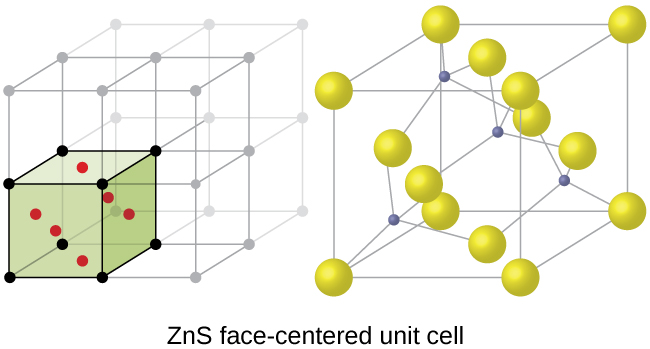
\includegraphics[width=0.9\textwidth,keepaspectratio]{media/zns_crystal_structure.jpg}
\caption{图15 立方ZnS型（闪锌矿）结构 — S2-面心立方密堆积，Zn2+填一半四面体空隙。注意Zn2+之间的位置关系——它们互相错开¼对角线}
\end{figure}

\paragraph{(4) 六方ZnS型（纤锌矿型，4:4配位）}\label{ux516dux65b9znsux578bux7ea4ux950cux77ffux578b44ux914dux4f4d}

{\def\LTcaptype{none} % do not increment counter
\begin{longtable}[]{@{}ll@{}}
\toprule\noalign{}
特征 & 描述 \\
\midrule\noalign{}
\endhead
\bottomrule\noalign{}
\endlastfoot
负离子堆积 & S\textsuperscript{2-} 按六方最密堆积 \\
正离子位置 & Zn\textsuperscript{2+} 占据一半正四面体空隙 \\
配位比 & 4:4 \\
晶胞内含 & 2 个 ZnS \\
实例 & ZnO、BeO、GaN、AlN \\
\end{longtable}
}

\subsubsection{3.3 其他常见结构}\label{ux5176ux4ed6ux5e38ux89c1ux7ed3ux6784}

\paragraph{\texorpdfstring{CaF\textsubscript{2}型（萤石型，8:4配位）}{CaF2型（萤石型，8:4配位）}}\label{caf2ux578bux8424ux77f3ux578b84ux914dux4f4d}

\begin{itemize}
\tightlist
\item
  Ca\textsuperscript{2+} 按面心立方排列
\item
  F\textsuperscript{-} 占据 Ca\textsuperscript{2+} 围成的\textbf{全部}正四面体空隙（8个）
\item
  配位比：Ca\textsuperscript{2+} 为 8 配位（不规则立方体配位），F\textsuperscript{-} 为 4 配位（正四面体）
\item
  实例：CaF\textsubscript{2}、BaF\textsubscript{2}、SrF\textsubscript{2}、UO\textsubscript{2}
\item
  \textbf{反萤石型}：正负离子位置互换------如 Li\textsubscript{2}O、Na\textsubscript{2}O（O\textsuperscript{2-} 按面心立方排列，Li\textsuperscript{+}/Na\textsuperscript{+} 填全部四面体空隙）
\end{itemize}

\paragraph{\texorpdfstring{TiO\textsubscript{2}型（金红石型，6:3配位）}{TiO2型（金红石型，6:3配位）}}\label{tio2ux578bux91d1ux7ea2ux77f3ux578b63ux914dux4f4d}

\begin{itemize}
\tightlist
\item
  Ti\textsuperscript{4+} 位于晶胞顶点和体心（四方晶系）
\item
  O\textsuperscript{2-} 位于 TiO\textsubscript{6} 八面体之间的共顶点连接
\item
  配位比：Ti\textsuperscript{4+} 为 6 配位（八面体），O\textsuperscript{2-} 为 3 配位（平面三角形配位）
\item
  实例：TiO\textsubscript{2}、MnO\textsubscript{2}、PbO\textsubscript{2}、SnO\textsubscript{2}
\end{itemize}

\subsubsection{3.4 结构类型对比总表}\label{ux7ed3ux6784ux7c7bux578bux5bf9ux6bd4ux603bux8868}

{\def\LTcaptype{none} % do not increment counter
\begin{longtable}[]{@{}
  >{\raggedright\arraybackslash}p{(\linewidth - 12\tabcolsep) * \real{0.1290}}
  >{\raggedright\arraybackslash}p{(\linewidth - 12\tabcolsep) * \real{0.1290}}
  >{\raggedright\arraybackslash}p{(\linewidth - 12\tabcolsep) * \real{0.1290}}
  >{\raggedright\arraybackslash}p{(\linewidth - 12\tabcolsep) * \real{0.1290}}
  >{\centering\arraybackslash}p{(\linewidth - 12\tabcolsep) * \real{0.1613}}
  >{\centering\arraybackslash}p{(\linewidth - 12\tabcolsep) * \real{0.1613}}
  >{\centering\arraybackslash}p{(\linewidth - 12\tabcolsep) * \real{0.1613}}@{}}
\toprule\noalign{}
\begin{minipage}[b]{\linewidth}\raggedright
结构类型
\end{minipage} & \begin{minipage}[b]{\linewidth}\raggedright
堆积离子
\end{minipage} & \begin{minipage}[b]{\linewidth}\raggedright
堆积方式
\end{minipage} & \begin{minipage}[b]{\linewidth}\raggedright
填隙离子
\end{minipage} & \begin{minipage}[b]{\linewidth}\centering
空隙类型
\end{minipage} & \begin{minipage}[b]{\linewidth}\centering
填隙率
\end{minipage} & \begin{minipage}[b]{\linewidth}\centering
配位比
\end{minipage} \\
\midrule\noalign{}
\endhead
\bottomrule\noalign{}
\endlastfoot
\textbf{CsCl} & Cl\textsuperscript{-} & 简单立方 & Cs\textsuperscript{+} & 立方体 & 100\% & 8:8 \\
\textbf{NaCl} & Cl\textsuperscript{-} & 面心立方(ccp) & Na\textsuperscript{+} & 正八面体 & 100\% & 6:6 \\
\textbf{立方ZnS} & S\textsuperscript{2-} & 面心立方(ccp) & Zn\textsuperscript{2+} & 正四面体 & 50\% & 4:4 \\
\textbf{六方ZnS} & S\textsuperscript{2-} & 六方(hcp) & Zn\textsuperscript{2+} & 正四面体 & 50\% & 4:4 \\
\textbf{CaF\textsubscript{2}} & Ca\textsuperscript{2+} & 面心立方(ccp) & F\textsuperscript{-} & 正四面体 & 100\% & 8:4 \\
\textbf{反萤石} & O\textsuperscript{2-} & 面心立方(ccp) & Li\textsuperscript{+} & 正四面体 & 100\% & 4:8 \\
\textbf{TiO\textsubscript{2}} & Ti\textsuperscript{4+} & 四方体心 & O\textsuperscript{2-} & 八面体链 & --- & 6:3 \\
\end{longtable}
}

\begin{quote}
📝 \textbf{练一练}：填写下表：
\end{quote}

{\def\LTcaptype{none} % do not increment counter
\begin{longtable}[]{@{}lccc@{}}
\toprule\noalign{}
结构类型 & 配位比 & 正离子空隙类型 & 填隙率 \\
\midrule\noalign{}
\endhead
\bottomrule\noalign{}
\endlastfoot
NaCl & ( ) & ( ) & ( ) \\
CsCl & ( ) & ( ) & ( ) \\
立方ZnS & ( ) & ( ) & ( ) \\
CaF\textsubscript{2} & ( ) & ( ) & ( ) \\
\end{longtable}
}

（答案见§九参考答案）

相关 KP：NaCl型结构 · CsCl型结构 · 立方ZnS型结构 · 六方ZnS型结构 · CaF2型结构 · NiAs型结构 · 反萤石型结构 · 金红石型结构

\begin{center}\rule{0.5\linewidth}{0.5pt}\end{center}

\subsection{四、半径比规则}\label{ux56dbux534aux5f84ux6bd4ux89c4ux5219}

\textbf{关联知识点}：离子半径 · 半径比规则

\subsubsection{4.1 离子晶体的''尺寸决定论''}\label{ux79bbux5b50ux6676ux4f53ux7684ux5c3aux5bf8ux51b3ux5b9aux8bba}

正离子填充什么类型的空隙------是四面体（4配位）、八面体（6配位）还是立方体（8配位）------这由什么决定？直觉告诉我们，\textbf{如果正离子太小，就填不进大的空隙；太大又会撑开负离子骨架}。半径比规则正是这一朴素直觉的量化表达。

\subsubsection{4.2 临界值几何推导}\label{ux4e34ux754cux503cux51e0ux4f55ux63a8ux5bfc}

半径比规则的核心思想：在纯离子模型中，正、负离子之间的静电吸引是最主要作用力。如果正离子太小，负离子外壳层就会互相接触------同种电荷相斥，结构不稳定。\textbf{最稳定的结构恰好是正离子刚好能接触到所有周围负离子的状态}------这就是''临界半径比''的几何原因。

\paragraph{\texorpdfstring{四配位（正四面体空隙）：\(r_+/r_- \geq 0.225\)}{四配位（正四面体空隙）：r\_+/r\_- \textbackslash geq 0.225}}\label{ux56dbux914dux4f4dux6b63ux56dbux9762ux4f53ux7a7aux9699r_r_--geq-0.225}

正四面体的几何关系：四个球在顶点，中心恰好放入一个刚好接触四个球的球。

设负离子半径 \(r_-\)，正离子半径 \(r_+\)，正四面体棱边长 \(a = 2r_-\)，体心到顶点距离 \(d = \frac{\sqrt{6}}{4}a = \frac{\sqrt{6}}{4} \cdot 2r_- = \frac{\sqrt{6}}{2}r_-\)

临界条件：\(d = r_- + r_+\) → \(r_+ = d - r_- = \left(\frac{\sqrt{6}}{2} - 1\right)r_-\) → \(\boxed{\frac{r_+}{r_-} = \frac{\sqrt{6}}{2} - 1 \approx 0.225}\)

\paragraph{\texorpdfstring{六配位（正八面体空隙）：\(r_+/r_- \geq 0.414\)}{六配位（正八面体空隙）：r\_+/r\_- \textbackslash geq 0.414}}\label{ux516dux914dux4f4dux6b63ux516bux9762ux4f53ux7a7aux9699r_r_--geq-0.414}

八面体xy平面截面为正方形：四个负离子在正方形顶点，正离子在中心。

正方形边长 \(a = 2r_-\)，对角线长 \(\sqrt{2}a = 2\sqrt{2}r_-\)，中心到顶点距离 \(= \frac{\sqrt{2}a}{2} = \sqrt{2}r_-\)

临界条件：\(\sqrt{2}r_- = r_- + r_+\) → \(r_+ = (\sqrt{2} - 1)r_-\) → \(\boxed{\frac{r_+}{r_-} = \sqrt{2} - 1 \approx 0.414}\)

\begin{figure}[H]\centering
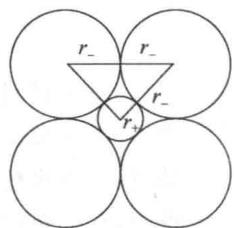
\includegraphics[width=0.9\textwidth,keepaspectratio]{media/octahedral-coordination-radius-ratio.jpg}
\caption{图16 八面体配位中正离子恰好嵌入空隙的临界条件——四个负离子构成正方形截面，正离子在中心刚好与四个负离子接触}
\end{figure}

\paragraph{\texorpdfstring{八配位（立方体空隙）：\(r_+/r_- \geq 0.732\)}{八配位（立方体空隙）：r\_+/r\_- \textbackslash geq 0.732}}\label{ux516bux914dux4f4dux7acbux65b9ux4f53ux7a7aux9699r_r_--geq-0.732}

立方体体对角线 = \(\sqrt{3}a\)，棱长 \(a = 2r_-\)，体对角线长 \(= 2\sqrt{3}r_-\)

中心到顶点距离 = \(\frac{2\sqrt{3}r_-}{2} = \sqrt{3}r_-\)

临界条件：\(\sqrt{3}r_- = r_- + r_+\) → \(r_+ = (\sqrt{3} - 1)r_-\) → \(\boxed{\frac{r_+}{r_-} = \sqrt{3} - 1 \approx 0.732}\)

\begin{figure}[H]\centering
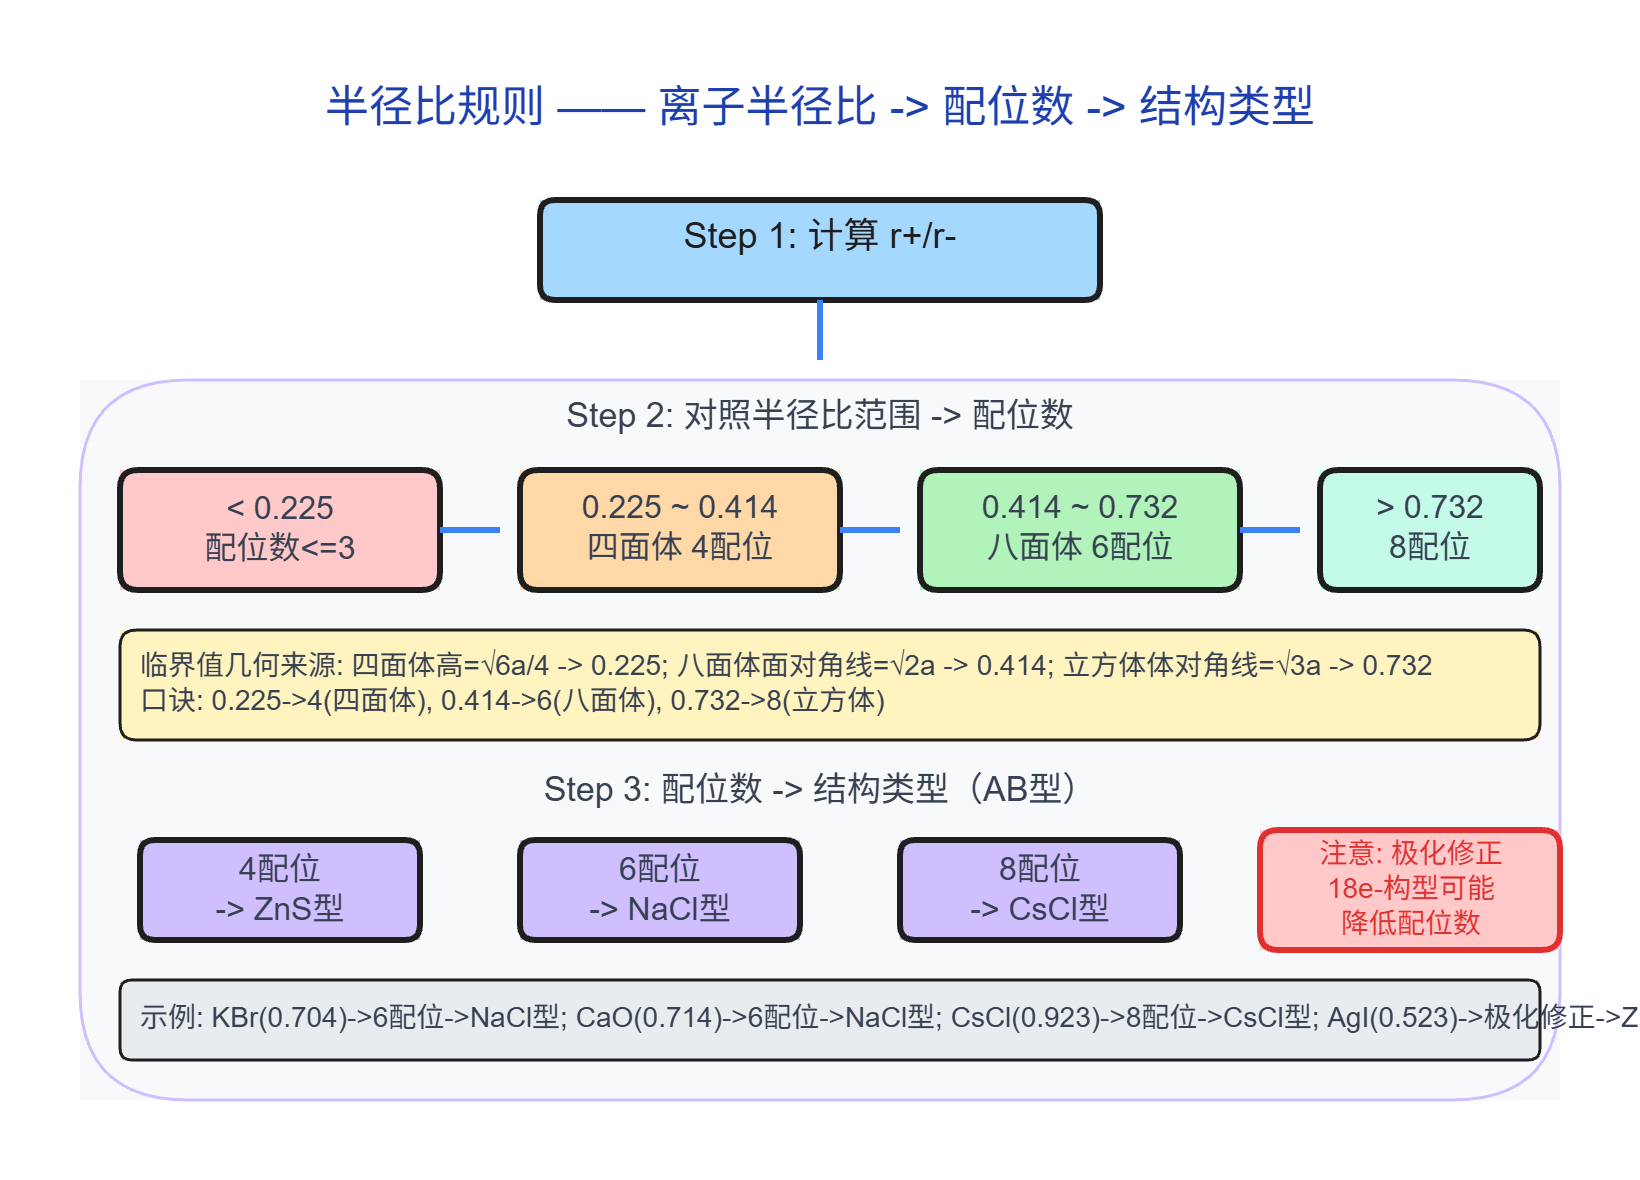
\includegraphics[width=0.9\textwidth,keepaspectratio]{media/半径比规则-配位数判断.决策图.png}
\caption{图17 半径比→配位数→结构类型判断决策图——三步法：算r₊/r₋→对照范围得配位数→推出结构类型}
\end{figure}

\subsubsection{4.3 半径比与配位数的关系}\label{ux534aux5f84ux6bd4ux4e0eux914dux4f4dux6570ux7684ux5173ux7cfb}

{\def\LTcaptype{none} % do not increment counter
\begin{longtable}[]{@{}cccl@{}}
\toprule\noalign{}
\(r_+/r_-\) 范围 & 可能配位数 & 空隙类型 & 典型结构 \\
\midrule\noalign{}
\endhead
\bottomrule\noalign{}
\endlastfoot
0.155 \textasciitilde{} 0.225 & 3 & 三角形 & --- \\
0.225 \textasciitilde{} 0.414 & 4 & 正四面体 & ZnS 型 \\
0.414 \textasciitilde{} 0.732 & 6 & 正八面体 & NaCl 型 \\
0.732 \textasciitilde{} 1.0 & 8 & 立方体 & CsCl 型 \\
≥ 1.0 & 12 & 金属堆积 & --- \\
\end{longtable}
}

\begin{quote}
🧠 \textbf{认知冲突}：「半径比规则是几何必要条件，不是充分条件」------rc/ra 在范围内只说明几何上允许这个配位数，但实际结构还受离子极化、共价成分、温度压力等因素影响。\textbf{AgI 的 rc/ra ≈ 0.51（NaCl型范围），但实际是ZnS型（4配位）}------因为Ag-I键有明显共价成分。
\end{quote}

\begin{quote}
⚠️ \textbf{易错点}：半径比规则给出的是\textbf{最小}半径比。若正离子半径比该临界值更小，正、负离子不能接触，结构不稳定。但半径比规则并非绝对------当离子极化显著时（共价成分增多），该规则的适用性下降。
\end{quote}

\begin{quote}
📝 \textbf{练一练}：已知离子半径（单位pm）：K\textsuperscript{+}=138, Ca\textsuperscript{2+}=100, Na\textsuperscript{+}=102, O\textsuperscript{2-}=140, Cl\textsuperscript{-}=181。判断：(1) KCl 的预期结构类型；(2) CaO 的预期结构类型。
（答案见§九参考答案）
\end{quote}

相关 KP：离子半径 · 半径比规则

\begin{center}\rule{0.5\linewidth}{0.5pt}\end{center}

\subsection{五、Pauling 规则与离子极化}\label{ux4e94pauling-ux89c4ux5219ux4e0eux79bbux5b50ux6781ux5316}

\textbf{关联知识点}：Pauling规则 · 离子极化 · 晶格能

\subsubsection{5.1 Pauling 电价规则------离子晶体结构的''电荷守恒''}\label{pauling-ux7535ux4ef7ux89c4ux5219ux79bbux5b50ux6676ux4f53ux7ed3ux6784ux7684ux7535ux8377ux5b88ux6052}

\textbf{问题}：在一个离子晶体中，正离子周围的负离子怎么排布才是最稳定的？Pauling 的第一规则（电价规则）给出了漂亮的答案：

\textbf{在稳定的离子晶体中，每个负离子的电价等于或近似等于从邻近正离子分配给该负离子的静电键强度的总和。}

\[
Z_- = \sum_i \frac{Z_{+,i}}{\text{CN}_i}
\]

其中 \(Z_-\) 为负离子的电荷，\(Z_{+,i}\) 为第 i 个正离子的电荷，\(\text{CN}_i\) 为正离子的配位数。

\begin{quote}
🗣️ \textbf{课堂原话}：``Pauling电价规则本质上是一本\textbf{能量账本}------每个正离子把自己'电力'平均分给所有邻居，所有邻居加起来必须刚好还完负离子的'债'。''
\end{quote}

\textbf{应用示例------判断NaCl型结构的合理性}：

NaCl型中，Cl\textsuperscript{-} 被 6 个 Na\textsuperscript{+} 包围（八面体配位）：
- 每个 Na\textsuperscript{+} 分配给 Cl\textsuperscript{-} 的静电键强度 = \(1/6\)
- 6 个 Na\textsuperscript{+} 总贡献 = \(6 \times 1/6 = 1\) = Cl\textsuperscript{-} 的电价 → \textbf{结构合理} ✅

\textbf{应用示例------判断CaF\textsubscript{2}型结构的合理性}：

Ca\textsuperscript{2+} 四面体配位（CN=8），F\textsuperscript{-} 四面体配位（CN=4）：
- 每个 Ca\textsuperscript{2+} 分配给 F\textsuperscript{-} 的静电键强度 = \(2/8 = 1/4\)
- 4 个 Ca\textsuperscript{2+} 对 F\textsuperscript{-} 总贡献 = \(4 \times 1/4 = 1\) = F\textsuperscript{-} 的电价 → \textbf{结构合理} ✅

\begin{figure}[H]\centering
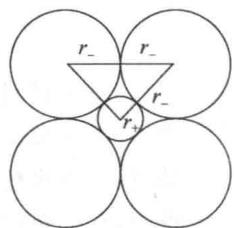
\includegraphics[width=0.9\textwidth,keepaspectratio]{media/13-12-octahedral-coordination.jpg}
\caption{图18 八面体配位结构 — 中心正离子与6个负离子配位，Pauling电价规则的典型应用场景}
\end{figure}

\begin{quote}
📝 \textbf{练一练}：采用 Pauling 电价规则检验 MgO（NaCl 型）的结构合理性。
（答案见§九参考答案）
\end{quote}

\subsubsection{5.2 Pauling 其他规则}\label{pauling-ux5176ux4ed6ux89c4ux5219}

\begin{itemize}
\tightlist
\item
  \textbf{第二规则（共顶点/共棱/共面规则）}：配位多面体倾向于共顶点连接，共棱和共面连接会降低稳定性（正离子间距减小，排斥增大）

  \begin{itemize}
  \tightlist
  \item
    共顶点 → 正离子间距最大，排斥最小
  \item
    共棱 → 中等
  \item
    共面 → 正离子间距最小，排斥最大
  \end{itemize}
\item
  \textbf{第三规则（规则性）}：配位多面体倾向于尽可能规则
\end{itemize}

\subsubsection{5.3 离子极化与 Fajans 规则}\label{ux79bbux5b50ux6781ux5316ux4e0e-fajans-ux89c4ux5219}

\paragraph{为什么有些离子晶体''不像离子晶体''？}\label{ux4e3aux4ec0ux4e48ux6709ux4e9bux79bbux5b50ux6676ux4f53ux4e0dux50cfux79bbux5b50ux6676ux4f53}

离子极化：\textbf{正离子使负离子电子云变形（极化作用），负离子被极化（变形性）}。当极化足够强时，键从离子型向共价型过渡------配位数下降、物性改变。

{\def\LTcaptype{none} % do not increment counter
\begin{longtable}[]{@{}lll@{}}
\toprule\noalign{}
因素 & 极化作用（正离子） & 变形性（负离子） \\
\midrule\noalign{}
\endhead
\bottomrule\noalign{}
\endlastfoot
电荷 & 电荷越高 → 极化越强 & 电荷越高 → 变形性越大 \\
半径 & 半径越小 → 极化越强 & 半径越大 → 变形性越大 \\
电子构型 & 18e\textsuperscript{-}/18+2e\textsuperscript{-} \textgreater{} 9\textasciitilde17e\textsuperscript{-} \textgreater{} 8e\textsuperscript{-} & 阴离子通常 \textgreater{} 阳离子 \\
\end{longtable}
}

\begin{quote}
🧠 \textbf{认知冲突}：「为什么AgI的半径比（0.523）落在NaCl型范围，实际却是ZnS型？」------Ag\textsuperscript{+}是18电子构型（4d\textsuperscript{10}），极化作用强；I\textsuperscript{-}半径大（220pm），变形性大。Ag\textsuperscript{+}的强极化使电子云严重畸变→键的共价性增大→配位数从6降为4。
\end{quote}

\begin{figure}[H]\centering
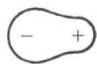
\includegraphics[width=0.9\textwidth,keepaspectratio]{media/13-17-ion-polarization-ideal-vs-polarized.jpg}
\caption{图19 离子极化效应示意 — 左：理想纯离子模型（电子云球对称）；右：极化后的电子云畸变（负离子电子云被正离子拉向一侧）}
\end{figure}

\textbf{经典反例}：

{\def\LTcaptype{none} % do not increment counter
\begin{longtable}[]{@{}
  >{\raggedright\arraybackslash}p{(\linewidth - 6\tabcolsep) * \real{0.2222}}
  >{\centering\arraybackslash}p{(\linewidth - 6\tabcolsep) * \real{0.2778}}
  >{\centering\arraybackslash}p{(\linewidth - 6\tabcolsep) * \real{0.2778}}
  >{\raggedright\arraybackslash}p{(\linewidth - 6\tabcolsep) * \real{0.2222}}@{}}
\toprule\noalign{}
\begin{minipage}[b]{\linewidth}\raggedright
化合物
\end{minipage} & \begin{minipage}[b]{\linewidth}\centering
预测结构（半径比规则）
\end{minipage} & \begin{minipage}[b]{\linewidth}\centering
实际结构
\end{minipage} & \begin{minipage}[b]{\linewidth}\raggedright
解释
\end{minipage} \\
\midrule\noalign{}
\endhead
\bottomrule\noalign{}
\endlastfoot
AgI & \(r_+/r_- = 115/220 = 0.523\) → NaCl 型（6配位） & ZnS 型（4配位） & Ag\textsuperscript{+} 为 18e\textsuperscript{-} 构型，极化作用强；I\textsuperscript{-} 半径大 → 共价性增强 → 配位数降低 \\
CuCl & \(r_+/r_- > 0.414\) → NaCl 型 & ZnS 型 & Cu\textsuperscript{+} 为 18e\textsuperscript{-} 构型，极化导致结构转变 \\
Al\textsubscript{2}O\textsubscript{3}（刚玉） & 预期较高配位 & 实际CN=6（八面体配位） & Al\textsuperscript{3+} 高电荷 + 小半径 → 极化力极强 \\
\end{longtable}
}

\begin{quote}
📝 \textbf{练一练}：解释为什么 BeO 采取六方 ZnS 型（4配位）而不是 NaCl 型（6配位）。已知 Be\textsuperscript{2+}半径31pm，O\textsuperscript{2-}半径140pm。
（答案见§九参考答案）
\end{quote}

相关 KP：Pauling规则 · 离子极化 · 晶格能 · 离子键

\begin{center}\rule{0.5\linewidth}{0.5pt}\end{center}

\subsection{六、其他晶体类型}\label{ux516dux5176ux4ed6ux6676ux4f53ux7c7bux578b}

\textbf{关联知识点}：原子晶体 · 分子晶体 · 金属晶体 · 金属键

\subsubsection{6.1 四大晶体类型对比}\label{ux56dbux5927ux6676ux4f53ux7c7bux578bux5bf9ux6bd4}

{\def\LTcaptype{none} % do not increment counter
\begin{longtable}[]{@{}
  >{\raggedright\arraybackslash}p{(\linewidth - 8\tabcolsep) * \real{0.2000}}
  >{\raggedright\arraybackslash}p{(\linewidth - 8\tabcolsep) * \real{0.2000}}
  >{\raggedright\arraybackslash}p{(\linewidth - 8\tabcolsep) * \real{0.2000}}
  >{\raggedright\arraybackslash}p{(\linewidth - 8\tabcolsep) * \real{0.2000}}
  >{\raggedright\arraybackslash}p{(\linewidth - 8\tabcolsep) * \real{0.2000}}@{}}
\toprule\noalign{}
\begin{minipage}[b]{\linewidth}\raggedright
晶体类型
\end{minipage} & \begin{minipage}[b]{\linewidth}\raggedright
结构单元
\end{minipage} & \begin{minipage}[b]{\linewidth}\raggedright
结合力
\end{minipage} & \begin{minipage}[b]{\linewidth}\raggedright
特点
\end{minipage} & \begin{minipage}[b]{\linewidth}\raggedright
实例
\end{minipage} \\
\midrule\noalign{}
\endhead
\bottomrule\noalign{}
\endlastfoot
\textbf{离子晶体} & 正负离子 & 离子键（静电作用） & 硬而脆、熔沸点高、水溶液导电、熔融导电 & NaCl、MgO、CaF\textsubscript{2} \\
\textbf{原子晶体（共价晶体）} & 原子 & 共价键 & 最硬、熔点最高、不导电（除少数）、耐腐蚀 & 金刚石、SiC、SiO\textsubscript{2} \\
\textbf{分子晶体} & 分子/原子 & 分子间力/氢键 & 软、熔沸点低、固态不导电 & 干冰、I\textsubscript{2}、冰、C\textsubscript{60} \\
\textbf{金属晶体} & 原子 & 金属键 & 导电导热、延展性好、有光泽 & Cu、Fe、Na、Al \\
\end{longtable}
}

\begin{figure}[H]\centering
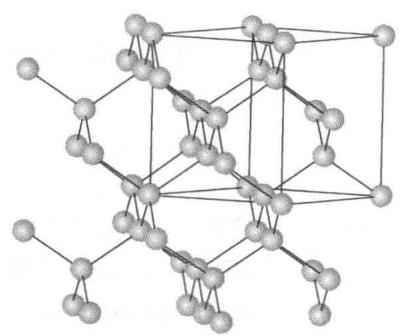
\includegraphics[width=0.9\textwidth,keepaspectratio]{media/diamond-structure.jpg}
\caption{图20 金刚石晶体结构（左）及其晶胞（右）— 每个C原子sp3杂化，四面体配位。金刚石是典型的原子晶体（共价晶体）}
\end{figure}

\begin{figure}[H]\centering
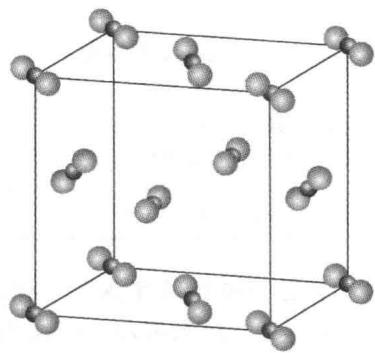
\includegraphics[width=0.9\textwidth,keepaspectratio]{media/13-14-co2-molecular-crystal-unit-cell.jpg}
\caption{图21 干冰（CO2）分子晶体晶胞 — 面心立方排列的CO2分子，分子之间以范德华力结合}
\end{figure}

\subsubsection{6.2 混合型晶体 ------ 石墨}\label{ux6df7ux5408ux578bux6676ux4f53-ux77f3ux58a8}

石墨为\textbf{层状结构}：
- 层内：C 原子 sp\textsuperscript{2} 杂化，形成离域π键（πₙᵐ），键能大 → \textbf{高熔点}
- 层间：范德华力结合 → \textbf{易滑动}（润滑性）
- 离域π电子可在层内自由移动 → \textbf{导电性}（各向异性：平行于层面导电性远好于垂直方向）

\textbf{各向异性的本质原因}：层内共价键（强方向性）+ 层间分子间力（弱非方向性）= 性质在不同方向上大不同。

\begin{figure}[H]\centering
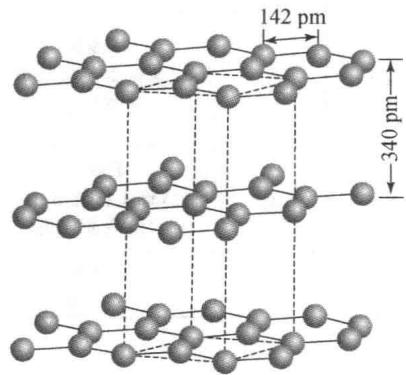
\includegraphics[width=0.9\textwidth,keepaspectratio]{media/graphite-structure.jpg}
\caption{图22 石墨的层状结构 — 层内共价键+离域π键（赋予高熔点和导电性），层间范德华力（赋予润滑性）}
\end{figure}

相关 KP：原子晶体 · 分子晶体 · 金属晶体 · 金属键 · 离子键 · 石墨结构 · 金刚石型结构 · 碳的同素异形体 · 二氧化硅结构 · 原子坐标参数 · 分数坐标

\begin{center}\rule{0.5\linewidth}{0.5pt}\end{center}

\subsection{七、典型例题}\label{ux4e03ux5178ux578bux4f8bux9898}

\subsubsection{例1 金属堆积 + 空间利用率 ⭐⭐}\label{ux4f8b1-ux91d1ux5c5eux5806ux79ef-ux7a7aux95f4ux5229ux7528ux7387}

\textbf{题目}：金属铜（Cu）采用面心立方堆积，已知 Cu 的原子半径为 128 pm，求晶胞参数 a 和晶体密度（Cu 的原子量 = 63.55 g/mol）。

\textbf{思路分析}：
1. 面心立方中面对角线方向原子接触 → \(\sqrt{2}a = 4r\)
2. 晶胞含 4 个 Cu 原子
3. 密度 \(\rho = n \times M / (N_A \times a^3)\)

\textbf{完整解答}：

\(a = \frac{4r}{\sqrt{2}} = \frac{4 \times 128}{\sqrt{2}} = 362\ \mathrm{pm}\)

\(V = a^3 = (362 \times 10^{-12}\ \mathrm{m})^3 = 4.74 \times 10^{-29}\ \mathrm{m}^3\)

\(\rho = \frac{4 \times 63.55}{6.022 \times 10^{23} \times (362 \times 10^{-12})^3} = 8.90\ \mathrm{g/cm}^3\)

\textbf{答案}：\(a = 362\ \mathrm{pm}\)，\(\rho = 8.90\ \mathrm{g/cm}^3\)

\begin{center}\rule{0.5\linewidth}{0.5pt}\end{center}

\subsubsection{例2 半径比规则 + 结构类型判断 ⭐⭐⭐}\label{ux4f8b2-ux534aux5f84ux6bd4ux89c4ux5219-ux7ed3ux6784ux7c7bux578bux5224ux65ad}

\textbf{题目}：已知离子半径如下（单位pm）：

{\def\LTcaptype{none} % do not increment counter
\begin{longtable}[]{@{}
  >{\centering\arraybackslash}p{(\linewidth - 18\tabcolsep) * \real{0.1000}}
  >{\centering\arraybackslash}p{(\linewidth - 18\tabcolsep) * \real{0.1000}}
  >{\centering\arraybackslash}p{(\linewidth - 18\tabcolsep) * \real{0.1000}}
  >{\centering\arraybackslash}p{(\linewidth - 18\tabcolsep) * \real{0.1000}}
  >{\centering\arraybackslash}p{(\linewidth - 18\tabcolsep) * \real{0.1000}}
  >{\centering\arraybackslash}p{(\linewidth - 18\tabcolsep) * \real{0.1000}}
  >{\centering\arraybackslash}p{(\linewidth - 18\tabcolsep) * \real{0.1000}}
  >{\centering\arraybackslash}p{(\linewidth - 18\tabcolsep) * \real{0.1000}}
  >{\centering\arraybackslash}p{(\linewidth - 18\tabcolsep) * \real{0.1000}}
  >{\centering\arraybackslash}p{(\linewidth - 18\tabcolsep) * \real{0.1000}}@{}}
\toprule\noalign{}
\begin{minipage}[b]{\linewidth}\centering
离子
\end{minipage} & \begin{minipage}[b]{\linewidth}\centering
K\textsuperscript{+}
\end{minipage} & \begin{minipage}[b]{\linewidth}\centering
Cs\textsuperscript{+}
\end{minipage} & \begin{minipage}[b]{\linewidth}\centering
Ca\textsuperscript{2+}
\end{minipage} & \begin{minipage}[b]{\linewidth}\centering
Na\textsuperscript{+}
\end{minipage} & \begin{minipage}[b]{\linewidth}\centering
Cl\textsuperscript{-}
\end{minipage} & \begin{minipage}[b]{\linewidth}\centering
Br\textsuperscript{-}
\end{minipage} & \begin{minipage}[b]{\linewidth}\centering
I\textsuperscript{-}
\end{minipage} & \begin{minipage}[b]{\linewidth}\centering
O\textsuperscript{2-}
\end{minipage} & \begin{minipage}[b]{\linewidth}\centering
S\textsuperscript{2-}
\end{minipage} \\
\midrule\noalign{}
\endhead
\bottomrule\noalign{}
\endlastfoot
半径 & 138 & 167 & 100 & 102 & 181 & 196 & 220 & 140 & 184 \\
\end{longtable}
}

判断下列化合物的晶体结构类型：(1) KBr；(2) CaO；(3) CsCl。

\textbf{思路分析}：
1. 计算 \(r_+/r_-\)
2. 对照半径比规则判断配位数和结构类型

\textbf{完整解答}：

\begin{enumerate}
\def\labelenumi{(\arabic{enumi})}
\item
  \textbf{KBr}：\(\frac{r_{\mathrm{K^+}}}{r_{\mathrm{Br^-}}} = \frac{138}{196} = 0.704\) → 0.414 \textless{} 0.704 \textless{} 0.732 → \textbf{NaCl型}
\item
  \textbf{CaO}：\(\frac{r_{\mathrm{Ca^{2+}}}}{r_{\mathrm{O^{2-}}}} = \frac{100}{140} = 0.714\) → 0.414 \textless{} 0.714 \textless{} 0.732 → \textbf{NaCl型}
\item
  \textbf{CsCl}：\(\frac{r_{\mathrm{Cs^+}}}{r_{\mathrm{Cl^-}}} = \frac{167}{181} = 0.923\) → 0.923 \textgreater{} 0.732 → \textbf{CsCl型}
\end{enumerate}

\begin{center}\rule{0.5\linewidth}{0.5pt}\end{center}

\subsubsection{例3 离子极化 + 结构反常 ⭐⭐⭐}\label{ux4f8b3-ux79bbux5b50ux6781ux5316-ux7ed3ux6784ux53cdux5e38}

\textbf{题目}：已知AgI中离子半径 Ag\textsuperscript{+}=115pm, I\textsuperscript{-}=220pm，按半径比规则应预测为哪种结构？实际AgI是哪种结构？为什么？

\textbf{思路分析}：
1. 先按半径比规则预测理论结构
2. 再考虑Ag\textsuperscript{+}的电子构型和I\textsuperscript{-}的变形性
3. 用离子极化理论解释偏差

\textbf{完整解答}：

\textbf{按半径比规则}：\(\frac{115}{220} = 0.523\) → 0.414 \textless{} 0.523 \textless{} 0.732 → 预测为\textbf{NaCl型}（6配位）

\textbf{实际结构}：AgI 为 \textbf{ZnS型}（4配位）

\textbf{原因分析}：
- Ag\textsuperscript{+} 为 \textbf{18电子构型}（\(4d^{10}\)），极化作用强
- I\textsuperscript{-} 半径大（220pm），\textbf{变形性大}
- Ag\textsuperscript{+} 的强极化作用使 I\textsuperscript{-} 电子云严重畸变 → 键的共价性显著增大
- 共价键具有方向性和饱和性 → 配位数从6降为4

\textbf{答案}：理论预测为NaCl型，实际为ZnS型；离子极化导致的键型过渡。

\begin{center}\rule{0.5\linewidth}{0.5pt}\end{center}

\subsubsection{例4 晶体类型综合判断 ⭐⭐}\label{ux4f8b4-ux6676ux4f53ux7c7bux578bux7efcux5408ux5224ux65ad}

\textbf{题目}：说明金刚石、NaCl、干冰（CO\textsubscript{2}）、铜四种晶体的键型、硬度、熔点差异，并解释原因。

\textbf{完整解答}：

{\def\LTcaptype{none} % do not increment counter
\begin{longtable}[]{@{}
  >{\raggedright\arraybackslash}p{(\linewidth - 10\tabcolsep) * \real{0.1538}}
  >{\raggedright\arraybackslash}p{(\linewidth - 10\tabcolsep) * \real{0.1538}}
  >{\raggedright\arraybackslash}p{(\linewidth - 10\tabcolsep) * \real{0.1538}}
  >{\centering\arraybackslash}p{(\linewidth - 10\tabcolsep) * \real{0.1923}}
  >{\centering\arraybackslash}p{(\linewidth - 10\tabcolsep) * \real{0.1923}}
  >{\raggedright\arraybackslash}p{(\linewidth - 10\tabcolsep) * \real{0.1538}}@{}}
\toprule\noalign{}
\begin{minipage}[b]{\linewidth}\raggedright
晶体
\end{minipage} & \begin{minipage}[b]{\linewidth}\raggedright
类型
\end{minipage} & \begin{minipage}[b]{\linewidth}\raggedright
键型
\end{minipage} & \begin{minipage}[b]{\linewidth}\centering
硬度
\end{minipage} & \begin{minipage}[b]{\linewidth}\centering
熔点
\end{minipage} & \begin{minipage}[b]{\linewidth}\raggedright
原因
\end{minipage} \\
\midrule\noalign{}
\endhead
\bottomrule\noalign{}
\endlastfoot
\textbf{金刚石} & 原子晶体 & 共价键（C-C） & \textbf{最硬} & \textbf{最高} & 三维网状共价键，键能大，方向性强 \\
\textbf{NaCl} & 离子晶体 & 离子键 & 中等 & 高 & 静电作用强，但不如共价键强 \\
\textbf{干冰} & 分子晶体 & 分子间力 & 软 & 最低（升华） & 分子间力很弱 \\
\textbf{铜} & 金属晶体 & 金属键 & 较低（延展性好） & 高 & 金属键无方向性，可滑移 \\
\end{longtable}
}

\textbf{硬度顺序}：金刚石 \textgreater{} NaCl \textgreater{} 铜 \textgreater{} 干冰

\subsubsection{例5 晶胞参数 + 空隙计算 ⭐⭐⭐}\label{ux4f8b5-ux6676ux80deux53c2ux6570-ux7a7aux9699ux8ba1ux7b97}

\textbf{题目}：已知金属Al采用面心立方堆积，晶胞参数 a = 405 pm。计算：
(1) Al的原子半径
(2) 每个晶胞中的四面体空隙数
(3) 假设把所有的四面体空隙填满H原子（H原子半径为 37 pm），H原子之间是否接触？

\textbf{完整解答}：

\begin{enumerate}
\def\labelenumi{(\arabic{enumi})}
\item
  面心立方：\(\sqrt{2}a = 4r\) → \(r = \frac{\sqrt{2}a}{4} = \frac{\sqrt{2} \times 405}{4} = 143\ \mathrm{pm}\)
\item
  每个fcc晶胞中有 8 个四面体空隙。
\item
  四面体空隙临界半径比：\(r_+/r_- \geq 0.225\)。H原子填Al的四面体空隙所需的临界半径 = \(0.225 \times 143 = 32.2\ \mathrm{pm}\)。H的半径37pm \textgreater{} 32.2pm → 几何上可以填入。
\end{enumerate}

但四面体空隙中填入H后，H原子的电子与Al\textsuperscript{3+}的排斥------实际上Al不形成氢化物。这个计算只是几何练习。

\begin{center}\rule{0.5\linewidth}{0.5pt}\end{center}

\subsubsection{\texorpdfstring{例6 CaF\textsubscript{2}结构分析 ⭐⭐}{例6 CaF2结构分析 ⭐⭐}}\label{ux4f8b6-caf2ux7ed3ux6784ux5206ux6790}

\textbf{题目}：CaF\textsubscript{2}（萤石）中 Ca\textsuperscript{2+} 半径为 100 pm，F\textsuperscript{-} 半径为 133 pm。
(1) 计算半径比，预测 Ca\textsuperscript{2+} 的配位数。
(2) 实际 CaF\textsubscript{2} 中 Ca\textsuperscript{2+} 的配位数和 F\textsuperscript{-} 的配位数各是多少？
(3) 一个 CaF\textsubscript{2} 晶胞含几个 Ca\textsuperscript{2+}？几个 F\textsuperscript{-}？

\textbf{完整解答}：

\begin{enumerate}
\def\labelenumi{(\arabic{enumi})}
\item
  \(r_+/r_- = 100/133 = 0.752 > 0.732\) → 预测配位数为 \textbf{8}。
\item
  实际 CaF\textsubscript{2} 中 Ca\textsuperscript{2+} 为 8 配位（立方体配位），F\textsuperscript{-} 为 4 配位（正四面体配位）。
\item
  Ca\textsuperscript{2+} 按面心立方排列：\(8 \times 1/8 + 6 \times 1/2 = 4\) 个
  F\textsuperscript{-} 占据全部8个正四面体空隙：\textbf{8} 个
  所以每个晶胞含 4 个 CaF\textsubscript{2}。
\end{enumerate}

\begin{center}\rule{0.5\linewidth}{0.5pt}\end{center}

\subsection{八、方法总结}\label{ux516bux65b9ux6cd5ux603bux7ed3}

\subsubsection{8.1 晶体结构分析流程图}\label{ux6676ux4f53ux7ed3ux6784ux5206ux6790ux6d41ux7a0bux56fe}

\begin{Shaded}
\begin{Highlighting}[]
\NormalTok{给定化学式}
\NormalTok{   ↓}
\NormalTok{Step 1: 判断晶体类型（离子/原子/分子/金属/混合）}
\NormalTok{   由组成元素和物性推断}
\NormalTok{   ↓}
\NormalTok{Step 2: 确定堆积方式（金属/离子晶体）}
\NormalTok{   AB 型 → 算半径比 → 对照范围 → 确定结构类型}
\NormalTok{   ↓}
\NormalTok{Step 3: 分析配位数和配位多面体}
\NormalTok{   NaCl: 6 配位八面体; CsCl: 8 配位立方体; ZnS: 4 配位四面体}
\NormalTok{   ↓}
\NormalTok{Step 4: 晶体密度计算}
\NormalTok{   ρ = (n × M) / (N\_A × a\^{}3\^{})}
\NormalTok{   关键：n → 晶胞中化学式单位数；a → 晶胞参数}
\NormalTok{   ↓}
\NormalTok{Step 5: 稳定性判断（必要时）}
\NormalTok{   半径比规则 → Pauling 电价规则 → 离子极化修正}
\end{Highlighting}
\end{Shaded}

\subsubsection{8.2 核心速查表}\label{ux6838ux5fc3ux901fux67e5ux8868}

{\def\LTcaptype{none} % do not increment counter
\begin{longtable}[]{@{}
  >{\raggedright\arraybackslash}p{(\linewidth - 4\tabcolsep) * \real{0.3333}}
  >{\raggedright\arraybackslash}p{(\linewidth - 4\tabcolsep) * \real{0.3333}}
  >{\raggedright\arraybackslash}p{(\linewidth - 4\tabcolsep) * \real{0.3333}}@{}}
\toprule\noalign{}
\begin{minipage}[b]{\linewidth}\raggedright
概念
\end{minipage} & \begin{minipage}[b]{\linewidth}\raggedright
关键公式/规律
\end{minipage} & \begin{minipage}[b]{\linewidth}\raggedright
注意点
\end{minipage} \\
\midrule\noalign{}
\endhead
\bottomrule\noalign{}
\endlastfoot
\textbf{7大晶系} & 轴长+轴角关系 & 六方注意120°；晶系由对称性定，不是边长 \\
\textbf{ccp空间利用率} & \(\pi/3\sqrt{2} \approx 74.05\%\) & 面对角线方向原子接触 \\
\textbf{bcc空间利用率} & \(\sqrt{3}\pi/8 \approx 68.02\%\) & 体对角线方向原子接触 \\
\textbf{hcp空间利用率} & \(\pi/3\sqrt{2} \approx 74.05\%\)（与ccp相同） & 理想轴比 c/a = 1.633 \\
\textbf{半径比规则} & 0.225→4, 0.414→6, 0.732→8 & 极化显著时规则失效 \\
\textbf{Pauling电价规则} & \(Z_- = \sum Z_+/ \text{CN}\) & 配位数不能加错 \\
\textbf{离子极化顺序} & 18e\textsuperscript{-} 构型 \textgreater{} 9\textasciitilde17e\textsuperscript{-} \textgreater{} 8e\textsuperscript{-} & AgI是经典反例 \\
\textbf{晶体密度} & \(\rho = nM/N_A a^3\) & 晶胞原子数 n 别数错 \\
\end{longtable}
}

\subsubsection{8.3 结构类型判断流程图}\label{ux7ed3ux6784ux7c7bux578bux5224ux65adux6d41ux7a0bux56fe}

\begin{Shaded}
\begin{Highlighting}[]
\NormalTok{给定 AB 型离子晶体}
\NormalTok{   ↓}
\NormalTok{计算 r₊/r₋}
\NormalTok{   ↓}
\NormalTok{┌─ \textless{}0.225 → 配位数3或更低（少见）}
\NormalTok{├─ 0.225\textasciitilde{}0.414 → 4配位 → ZnS型}
\NormalTok{├─ 0.414\textasciitilde{}0.732 → 6配位 → NaCl型}
\NormalTok{├─ 0.732\textasciitilde{}1.0 → 8配位 → CsCl型}
\NormalTok{└─ \textgreater{}1.0 → 配位数12 → 金属堆积}
\NormalTok{   ↓}
\NormalTok{是否有强极化？(Ag\^{}+\^{}, Cu\^{}+\^{}, Zn\^{}2+\^{}, Cd\^{}2+\^{}等)}
\NormalTok{  → 是：配位数可能下降（→ ZnS型或更低）}
\NormalTok{  → 否：按半径比规则预测}
\end{Highlighting}
\end{Shaded}

\begin{center}\rule{0.5\linewidth}{0.5pt}\end{center}

\subsection{九、练习题}\label{ux4e5dux7ec3ux4e60ux9898}

\subsubsection{9.1 基础巩固}\label{ux57faux7840ux5de9ux56fa}

\begin{enumerate}
\def\labelenumi{\arabic{enumi}.}
\tightlist
\item
  说出立方晶系、四方晶系、六方晶系的轴长/轴角特征。
\item
  计算面心立方（fcc）一个晶胞中的原子数，已知原子位于顶点和面心。
\item
  已知 CsCl 型晶体中 Cl\textsuperscript{-} 和 Cs\textsuperscript{+} 的坐标分别是 (0,0,0) 和 (½,½,½)，计算一个晶胞含多少个 CsCl 化学式单位。
\item
  已知 Na\textsuperscript{+} 半径为 102 pm，Cl\textsuperscript{-} 半径为 181 pm，判断 NaCl 的晶体结构类型和配位数。
\item
  背诵半径比规则的三档临界值。
\end{enumerate}

\subsubsection{9.2 提高训练}\label{ux63d0ux9ad8ux8badux7ec3}

\begin{enumerate}
\def\labelenumi{\arabic{enumi}.}
\setcounter{enumi}{5}
\tightlist
\item
  已知 Ca\textsuperscript{2+} 半径为 100 pm，F\textsuperscript{-} 半径为 133 pm，判断 CaF\textsubscript{2} 中 Ca\textsuperscript{2+} 的配位数。
\item
  解释为什么 AgI 采取 ZnS 型（4配位）而非 NaCl 型（6配位）。
\item
  已知 MgO（NaCl型）和 NaF（NaCl型）具有相同结构，但 MgO 的熔点（2852°C）远高于 NaF（993°C），解释原因。
\item
  采用 Pauling 电价规则检验 MgO（NaCl 型）的结构合理性。
\item
  推导 hcp 的理想轴比 c/a。
\item
  fcc 晶胞中有多少个八面体空隙？多少个四面体空隙？验证''每球对应1个八面体空隙+2个四面体空隙''。
\item
  已知 Be\textsuperscript{2+}=31pm, O\textsuperscript{2-}=140pm，判断 BeO 的预期结构。如果实际 BeO 为 ZnS 型，为什么？
\end{enumerate}

\subsubsection{9.3 挑战题}\label{ux6311ux6218ux9898}

\begin{enumerate}
\def\labelenumi{\arabic{enumi}.}
\setcounter{enumi}{12}
\tightlist
\item
  Cu 的晶体结构为面心立方，原子半径为 128 pm，原子量为 63.55，计算 Cu 的理论密度。若实验测得密度为 8.96 g/cm\textsuperscript{3}，计算 Cu 晶体中实际晶胞参数是多少？
\item
  NiAs 型结构（NiAs，红镍矿）是另一种常见 AB 型结构------As 按六方密堆积(hcp)，Ni 填满全部八面体空隙。写出 Ni 的配位数和 As 的配位数，并画出结构示意。
\item
  某 AB\textsubscript{2} 型离子晶体，A\textsuperscript{2+} 半径 110 pm，B\textsuperscript{-} 半径 200 pm。预测其可能的结构类型，画出晶胞示意并计算每个晶胞中的化学式单位数。
\end{enumerate}

\begin{center}\rule{0.5\linewidth}{0.5pt}\end{center}

\subsection{参考答案与提示}\label{ux53c2ux8003ux7b54ux6848ux4e0eux63d0ux793a}

\subsubsection{§一 练一练}\label{ux4e00-ux7ec3ux4e00ux7ec3}

\(\gamma = 120^\circ\) → 该条件属于六方晶系特征。且 \(a = b \neq c\) → \textbf{六方晶系} ✅

\subsubsection{§二 练一练}\label{ux4e8c-ux7ec3ux4e00ux7ec3}

hcp 中，密置双层中上层球落在下层三个球形成的凹陷处。三个下层球的球心构成正三角形，边长 \(2r\)。上层球球心到三个下层球球心的距离相等，构成正四面体。正四面体高 \(h = \frac{\sqrt{6}}{3} \times 2r\)。所以两层间的垂直距离 = 正四面体的高 = \(\frac{2\sqrt{6}}{3}r\)。一个 hcp 晶胞的 c 轴包含 2 层（即 AB 两个底面的垂直距离 × 2）：\(c = 2 \times \frac{2\sqrt{6}}{3}r = \frac{4\sqrt{6}}{3}r = 4\sqrt{\frac{2}{3}}r\)。而 \(a = 2r\)，所以 \(c/a = 2\sqrt{\frac{2}{3}} \approx 1.633\) ✅

\subsubsection{§三 练一练}\label{ux4e09-ux7ec3ux4e00ux7ec3}

{\def\LTcaptype{none} % do not increment counter
\begin{longtable}[]{@{}lccc@{}}
\toprule\noalign{}
结构类型 & 配位比 & 正离子空隙类型 & 填隙率 \\
\midrule\noalign{}
\endhead
\bottomrule\noalign{}
\endlastfoot
NaCl & 6:6 & 正八面体空隙 & 100\% \\
CsCl & 8:8 & 立方体空隙 & 100\% \\
立方ZnS & 4:4 & 正四面体空隙 & 50\% \\
CaF\textsubscript{2} & 8:4 & 正四面体空隙 & 100\%（Ca\textsuperscript{2+}为骨架） \\
\end{longtable}
}

\subsubsection{§四 练一练}\label{ux56db-ux7ec3ux4e00ux7ec3}

\begin{enumerate}
\def\labelenumi{(\arabic{enumi})}
\item
  \textbf{KCl}：\(r_+/r_- = 138/181 = 0.762\)，0.732 \textless{} 0.762 \textless{} 1.0 → 预测为 \textbf{CsCl型}（实际上 KCl 在常温下也是 NaCl 型！------这就是''半径比规则是必要条件而非充分条件''的例证。KCl 的真实结构是 NaCl 型，因为 KCl 的离子极化程度较低，倾向于更稳定的 NaCl 排列)。
\item
  \textbf{CaO}：\(r_+/r_- = 100/140 = 0.714\)，0.414 \textless{} 0.714 \textless{} 0.732 → \textbf{NaCl型} ✅
\end{enumerate}

\subsubsection{§五 练一练}\label{ux4e94-ux7ec3ux4e00ux7ec3}

MgO 为 NaCl 型，Mg\textsuperscript{2+} 被 6 个 O\textsuperscript{2-} 包围。
每个 Mg\textsuperscript{2+} 分配静电键强度 = \(2/6 = 1/3\)，
6 个 Mg\textsuperscript{2+} 对 O\textsuperscript{2-} 总贡献 = \(6 \times 1/3 = 2\) = O\textsuperscript{2-} 的电价 → \textbf{结构合理} ✅

\subsubsection{§五 练一练（极化）}\label{ux4e94-ux7ec3ux4e00ux7ec3ux6781ux5316}

Be\textsuperscript{2+} 半径 31pm，电荷 +2 → \textbf{电荷密度极高}（极化作用极强）。O\textsuperscript{2-} 半径 140pm，变形性大。两者之间已经发生了从离子键到共价键的显著过渡，因此 BeO 的实际配位数为 4（六方 ZnS 型），而非半径比规则预测的 NaCl 型（6配位）。

\subsubsection{9.1 基础巩固}\label{ux57faux7840ux5de9ux56fa-1}

\begin{enumerate}
\def\labelenumi{\arabic{enumi}.}
\item
  \textbf{立方}：\(a=b=c, \alpha=\beta=\gamma=90^\circ\)；\textbf{四方}：\(a=b\neq c, \alpha=\beta=\gamma=90^\circ\)；\textbf{六方}：\(a=b\neq c, \alpha=\beta=90^\circ, \gamma=120^\circ\)。
\item
  顶点 \(8 \times 1/8 = 1\)，面心 \(6 \times 1/2 = 3\)，共 \textbf{4个原子}。
\item
  顶点 8 个 Cl\textsuperscript{-} 各贡献 1/8 = 1 个 Cl\textsuperscript{-}，体心 1 个 Cs\textsuperscript{+} → \textbf{1个} CsCl。
\item
  \(r_+/r_- = 102/181 = 0.564\)，0.414 \textless{} 0.564 \textless{} 0.732 → \textbf{NaCl型}，配位数 \textbf{6}。
\item
  0.225（四面体）、0.414（八面体）、0.732（立方体）。
\end{enumerate}

\subsubsection{9.2 提高训练}\label{ux63d0ux9ad8ux8badux7ec3-1}

\begin{enumerate}
\def\labelenumi{\arabic{enumi}.}
\setcounter{enumi}{5}
\item
  \(r_+/r_- = 100/133 = 0.752 > 0.732\) → Ca\textsuperscript{2+} 配位数为 \textbf{8}（CaF\textsubscript{2} 萤石型，实际配位比 8:4）。
\item
  \textbf{提示}：Ag\textsuperscript{+} 为 18 电子构型，极化作用强；I\textsuperscript{-} 半径大、变形性大。强极化导致键共价性增大，配位数从 6 降为 4（ZnS 型）。
\item
  MgO 中 Mg\textsuperscript{2+} 和 O\textsuperscript{2-} 电荷均为 \(\pm2\)，NaF 中 Na\textsuperscript{+} 和 F\textsuperscript{-} 电荷均为 \(\pm1\)。晶格能 \(U \propto Z_+Z_-/r\)，电荷效应对晶格能的贡献远大于半径差异 → MgO 晶格能远大于 NaF → 熔点更高。
\item
  MgO 为 NaCl 型，Mg\textsuperscript{2+} 被 6 个 O\textsuperscript{2-} 包围。每个 Mg\textsuperscript{2+} 分配静电键强度 = \(2/6 = 1/3\)，6 个总贡献 = \(6 \times 1/3 = 2\) = O\textsuperscript{2-} 的电价 → \textbf{结构合理} ✅
\item
  \textbf{hcp 理想 c/a}：\(c/a = 2\sqrt{2/3} \approx 1.633\)。推导：正四面体高 \(h = \sqrt{6}/3 \times a\)，hcp 单层高 \(= 2h\)，\(c = 2 \times 2h = 4h\) → \(c/a = 2\sqrt{2/3}\)。
\item
  fcc 有 \textbf{4个八面体空隙} + \textbf{8个四面体空隙}。验证：每球周围有 6 个八面体空隙，每个由6个球共享 → \(6 \times 4 / 6 = 4\) ✅。每球周围有 8 个四面体空隙，每个由4个球共享 → \(8 \times 4 / 4 = 8\) ✅。
\item
  Be\textsuperscript{2+}/O\textsuperscript{2-} 半径比 = 31/140 = 0.221，本应在 4 配位范围但非常接近下限。实际 BeO 为 ZnS 型（4配位）------原因：Be\textsuperscript{2+} 电荷高、半径极小 → 极化力极强 → 共价性显著 → 4配位被锁定。
\end{enumerate}

\subsubsection{9.3 挑战题}\label{ux6311ux6218ux9898-1}

\begin{enumerate}
\def\labelenumi{\arabic{enumi}.}
\setcounter{enumi}{12}
\item
  \textbf{提示}：理论密度 \(\rho_{th} = 4 \times 63.55 / (N_A \times a^3)\)，\(a = 4r/\sqrt{2} = 362\ \mathrm{pm}\)。\(\rho_{th} \approx 8.90\ \mathrm{g/cm}^3\)。由实验密度反推晶胞参数：\(a_{exp} = \left(\frac{4 \times 63.55}{6.022 \times 10^{23} \times 8.96}\right)^{1/3}\)，注意单位换算。
\item
  NiAs 型：As 按 hcp 堆积，Ni 填全部八面体空隙。Ni 的配位数 = 6（八面体），As 的配位数 = 6（三棱柱配位，每个 As 周围有 6 个 Ni）。晶胞中化学式比 1:1。
\item
  \(r_+/r_- = 110/200 = 0.55\)，在 0.414\textasciitilde0.732 范围 → 配位数 6。可能的 AB\textsubscript{2} 型结构有：金红石型（TiO\textsubscript{2}，四面体，配位比 6:3）。CaF\textsubscript{2} 型的 \(r_+/r_-\) 要求 \textgreater{} 0.732，这里不满足。所以预测为 \textbf{金红石型}。
\end{enumerate}

\begin{center}\rule{0.5\linewidth}{0.5pt}\end{center}

\subsection{延伸阅读}\label{ux5ef6ux4f38ux9605ux8bfb}

\begin{itemize}
\tightlist
\item
  专题-晶体与配合物深化 --- 专题页：核心结论与解题套路
\item
  专题-晶体结构计算 --- 晶体结构计算题的专题整理
\item
  2026-06-23-晶体学基础（讲义）--- 点阵与晶系的详细展开
\item
  2026-06-23-金属键与金属晶体（讲义）--- 金属堆积的完整推导
\item
  2026-06-23-离子键与离子晶体（讲义）--- Born-Haber 循环与晶格能
\item
  2026-06-23-其他类型晶体（讲义）--- 原子/分子/混合型晶体的系统介绍
\item
  12-教学洞察/教学洞察-晶体结构基础 --- 教学决策支持：认知冲突、类比、高频错误
\item
  Pauling规则 --- 电价规则详解与更多实例
\item
  离子极化 --- Fajans 规则的应用拓展
\item
  密堆积 --- 三种主要堆积方式的KP级完整推导
\item
  NaCl型结构 · CsCl型结构 · 立方ZnS型结构 · CaF2型结构
\item
  宋天佑《无机化学》§10-11 章
\item
  《化学竞赛初赛讲义》第 7 讲 --- 晶体结构
\end{itemize}

\begin{center}\rule{0.5\linewidth}{0.5pt}\end{center}
